\thispagestyle{duongvaotoanhocnone}
\pagestyle{duongvaotoanhoc}
\everymath{\color{duongvaotoanhoc}}
\graphicspath{{../duongvaotoanhoc/pic/}}
\blfootnote{$^*$\color{duongvaotoanhoc}Nguồn: Math Horizons $02/2015$.}
\blfootnote{$^1$\color{duongvaotoanhoc}Viện Toán học.}
\begingroup
\AddToShipoutPicture*{\put(0,616){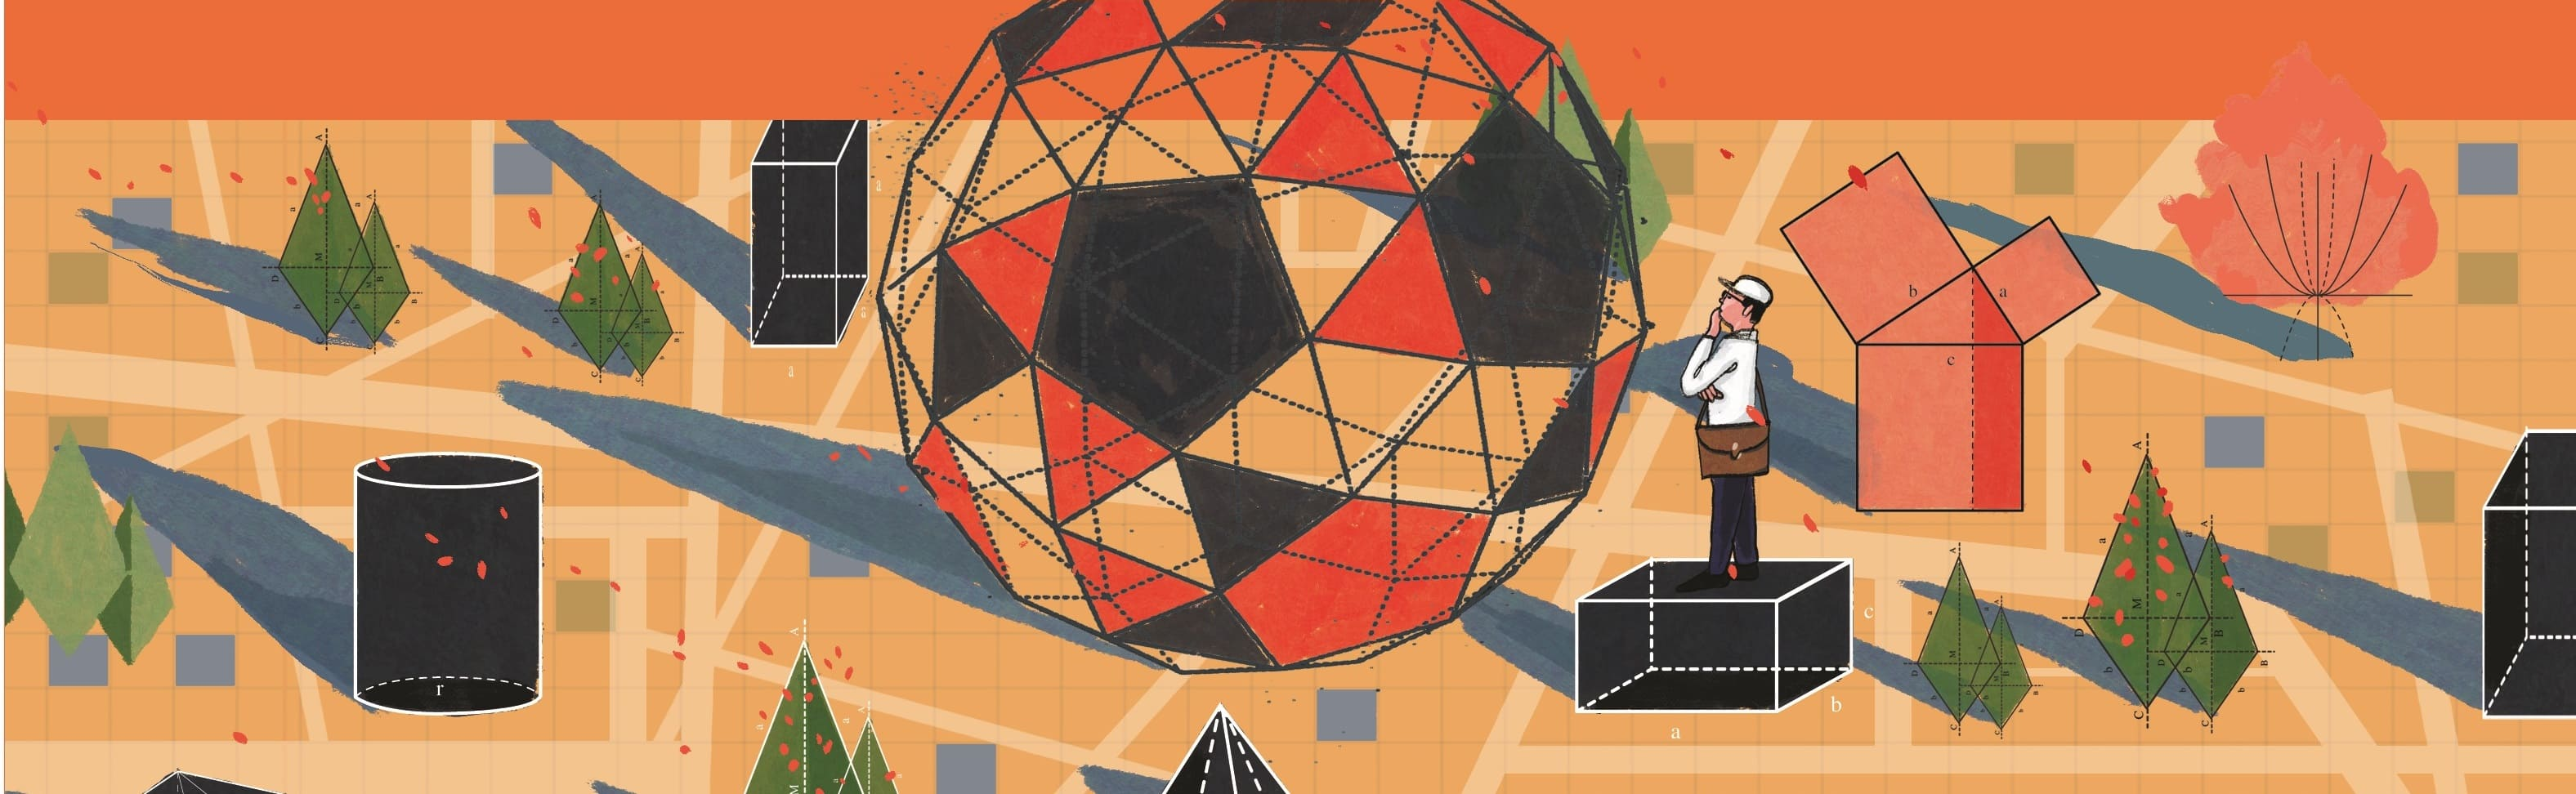
\includegraphics[width=19.3cm]{../bannerduongvao}}}
\AddToShipoutPicture*{\put(87,530){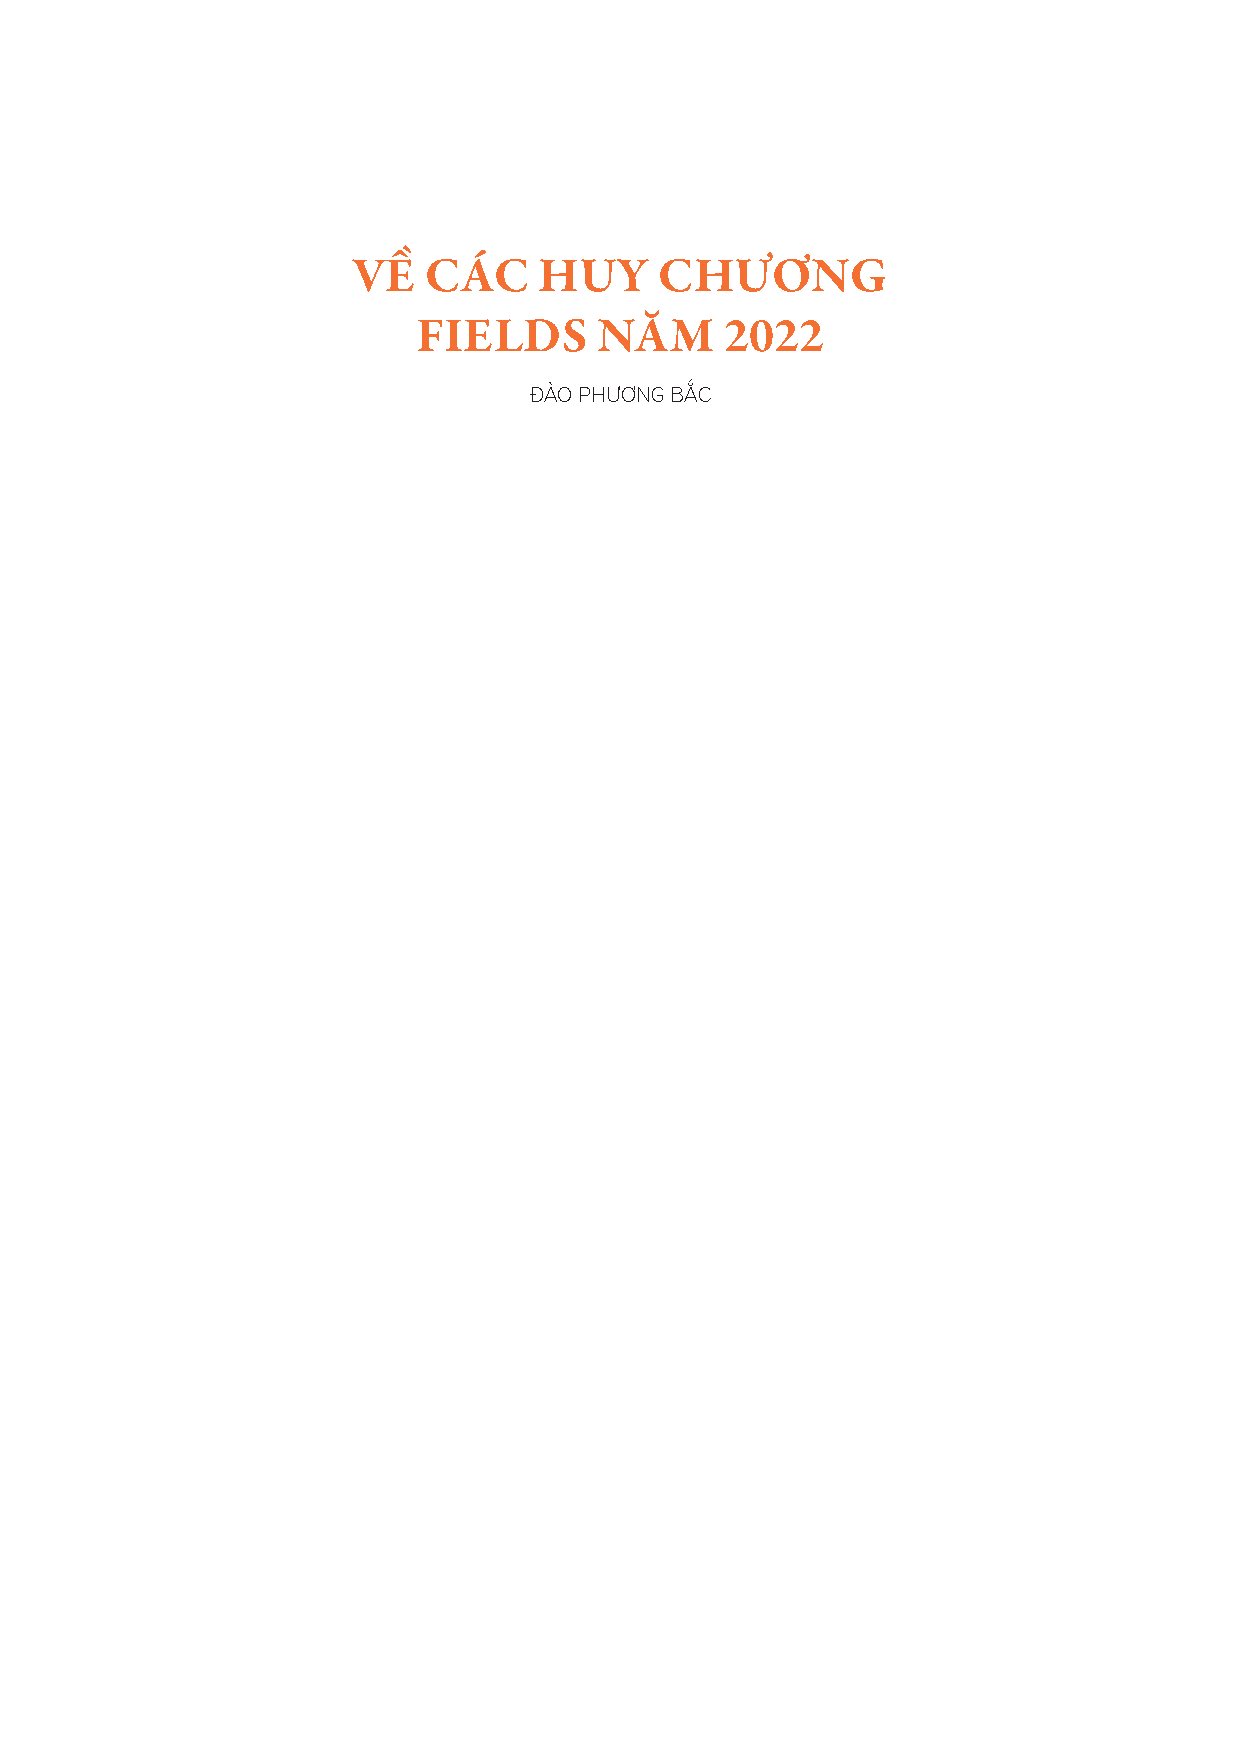
\includegraphics[scale=0.98]{../tieude.pdf}}}
\centering
\endgroup

\vspace*{180pt}

\begin{multicols}{2}	
	Khi minh họa cho các ứng dụng của toán học trong thực tế, thật khó tìm được chủ đề nào tốt hơn môn bi--a. Các đồ vật liên quan rất đơn giản: một cái bàn và một quả bóng \linebreak bi--a (và một cái que cơ để đánh quả bóng đi, nhưng vì nó không đóng vai trò gì sau này, chúng ta sẽ bỏ qua nó). 
	\vskip 0.1cm
	Từ quan điểm của một nhà toán học, chỉ có hai nguyên tắc vật lý cơ bản: Quả bóng di chuyển theo một đường thẳng cho đến khi nó chạm vào cạnh bàn, tại đó, chỉ nó tuân theo quy tắc rằng góc tới bằng góc phản xạ. Không cần phải bận tâm tới ma sát, độ quay, hoặc các vấn đề rắc rối khác.
	\vskip 0.1cm
	Thực hiện quá trình đơn giản hóa này đến mức tối giản, chúng ta coi bàn bi--a như một đa giác trong mặt phẳng và quả bóng là một điểm chuyển động theo các quy tắc đã nêu trên. Đường đi của bóng được gọi là \emph{đường đi bi--a}. 
	\vskip 0.1cm
	Trong khi một người chơi bi--a muốn biết làm sao đưa được bóng đến một vị trí cụ thể trên bàn thì nhà toán học đặt câu hỏi: Nếu chúng ta đánh quả bóng theo một hướng cho trước, đâu là những nơi mà một lúc nào đó quả bóng sẽ đi qua? Trong bối cảnh này, \linebreak bi--a là một \emph{hệ động lực}. Vị trí và hướng đi của quả bóng thay đổi theo thời gian, và chúng ta quan tâm đến dáng điệu dài hạn trong chuyển động của nó.
	\vskip 0.1cm
	Để đơn giản hóa cuộc thảo luận, chúng ta sẽ tập trung vào câu hỏi về những đường  bi--a nào là \emph{tuần hoàn}: Tức là, vị trí và hướng đi ban đầu của quả bóng bi--a như thế nào để khiến nó quay trở lại vị trí ban đầu, theo cùng một hướng như khi xuất phát, và cứ mãi lặp lại cùng một đường đi như vậy?
	\vskip 0.1cm
	Có lẽ sẽ không có gì ngạc nhiên khi câu trả lời cho câu hỏi này phụ thuộc vào vị trí và hướng chuyển động ban đầu của quả bóng. Cũng không có gì ngạc nhiên khi câu trả lời phụ thuộc vào hình dạng của cái bàn bi--a. Chúng ta sẽ bắt đầu với bàn bi--a có hình dạng quen thuộc nhất, hình chữ nhật, sau đó là đến hình tam giác.
	\vskip 0.1cm
	{\bf\color{duongvaotoanhoc}Bàn bi--a chữ nhật}
	\vskip 0.1cm
	Bi--a thông thường được chơi trên bàn hình chữ nhật. Bàn kích thước tiêu chuẩn có tỷ lệ độ dài cạnh là $2:1$, nhưng ở đây chúng ta cho phép bàn có kích thước $a\times b$ bất kỳ. Trên một bàn bất kỳ như vậy, luôn có một số đường đi tuần hoàn hiển nhiên:
	chẳng hạn như, một quả bóng nảy qua lại giữa hai cạnh đối diện nhau và vuông góc với chúng.
	\vskip 0.1cm
	Mày mò một chút, chúng ta tìm được các đường đi tuần hoàn khác: hình thoi nối trung điểm của các cạnh bàn, hay chẳng hạn như đường đi dích dắc chạm vào một cặp cạnh mỗi bên ba lần, và cặp còn lại mỗi bên hai lần như trong Hình $1$. Có điều gì chung cho những
	đường đi này mà chúng ta có thể tổng quát lên để tìm tất cả các đường đi tuần hoàn?
	\begin{figure}[H]
		\vspace*{-5pt}
		\centering
		\captionsetup{labelformat= empty, justification=centering}
		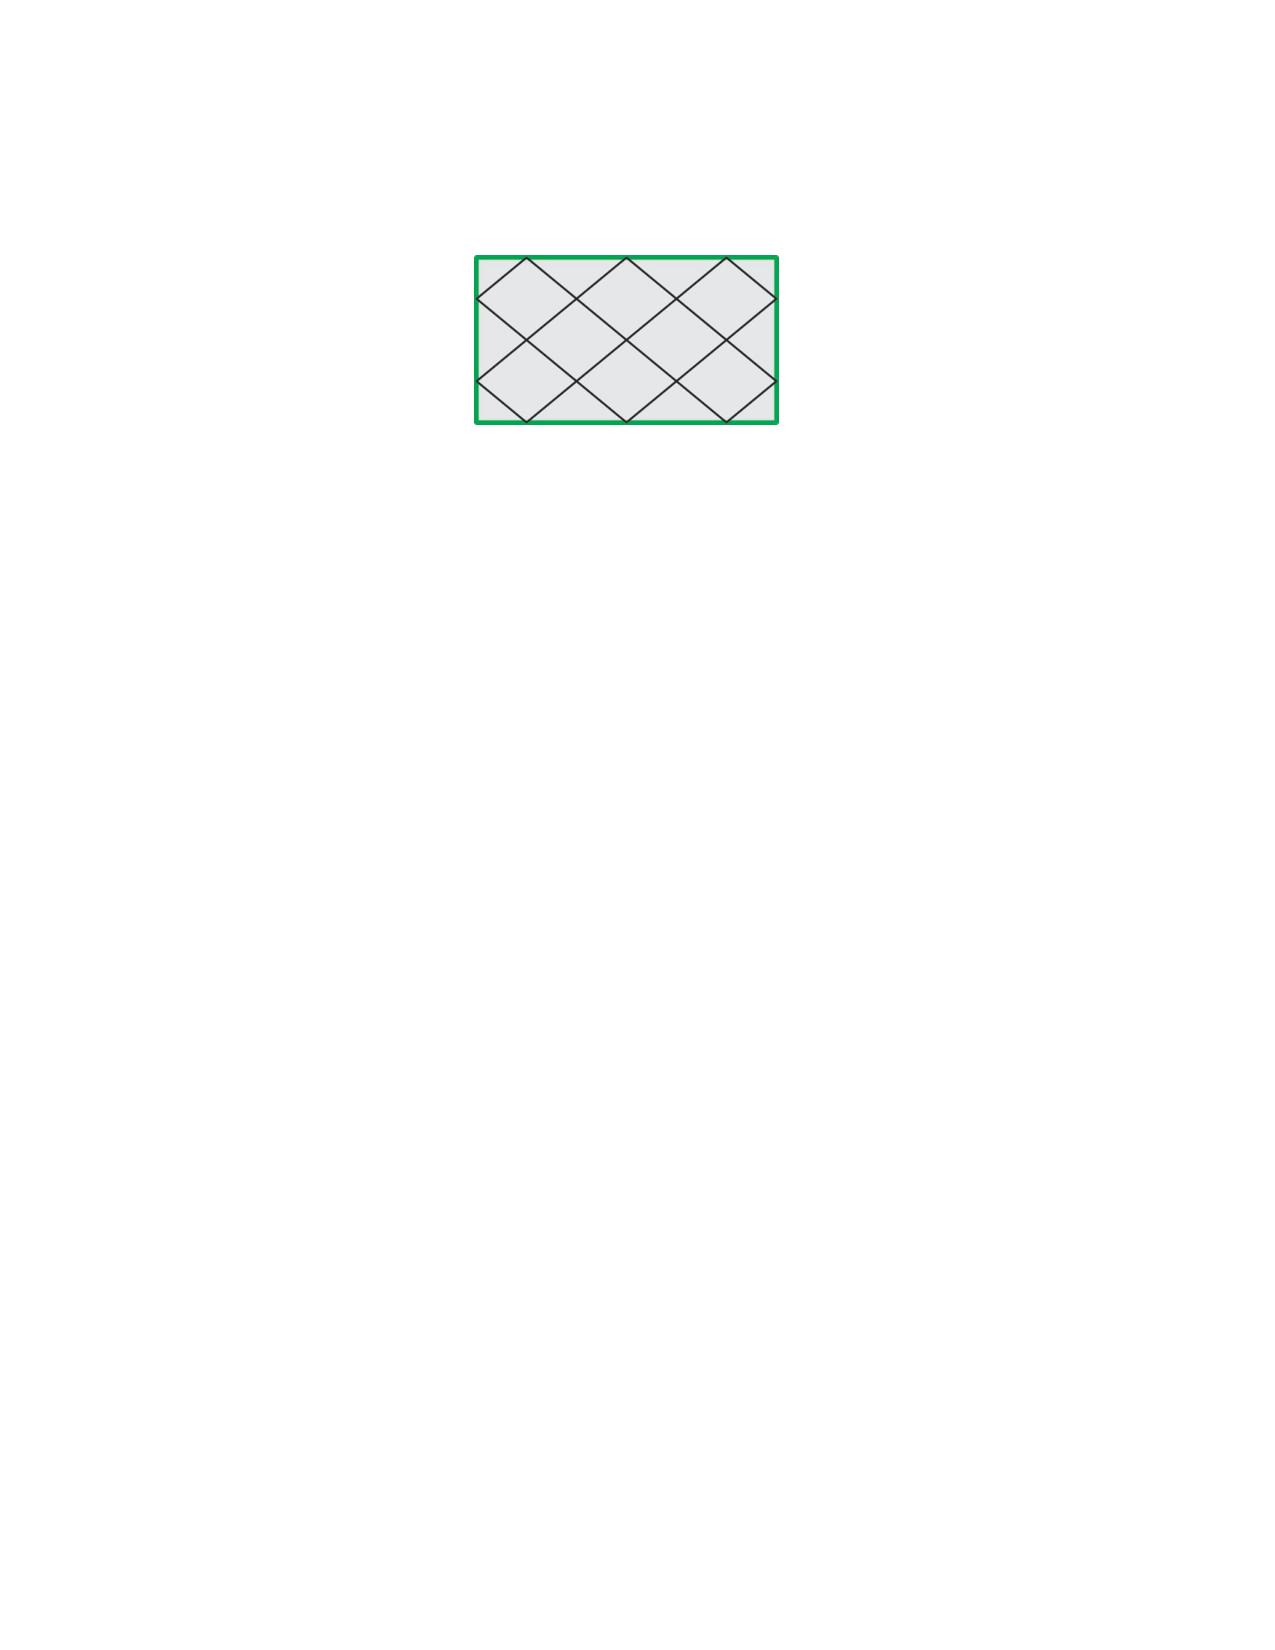
\includegraphics[width= 1\linewidth]{1}
		\caption{\small\textit{\color{duongvaotoanhoc}Hình $1$. Một đường đi bi--a tuần hoàn trong hình chữ nhật.}}
		\vspace*{-10pt}
	\end{figure}
	Bất kỳ đường đi bi--a nào quay trở lại vị trí và hướng đi ban đầu của nó phải đi theo phương ngang của hình chữ nhật một số chẵn lần, giả sử là $2N$ (lý do là vì quả bóng đổi hướng chuyển động  từ trái sang phải, hoặc phải sang trái, mỗi khi nó nảy tại một trong các cạnh thẳng đứng của bàn). Tương tự như vậy, nó phải đi theo phương dọc của hình chữ nhật một số chẵn lần, giả sử là $2M$. Cho trước một cặp số nguyên chẵn không âm tùy ý $(2N, 2M)$, liệu chúng ta có thể tìm được một đường đi tuần hoàn với số lần đi như vậy?
	\vskip 0.1cm
	Hãy thực hiện cách tiếp cận ``qua gương" để tìm một đường đi như vậy. Hãy coi đường đi bi--a như một tia sáng. Thay vì lấy mỗi cạnh của hình chữ nhật là một tấm gương, hãy coi nó như một tấm kính, và khi đến đó, tia sáng tiếp tục đi theo một đường thẳng xuyên vào một bản sao đối xứng của hình chữ nhật ban đầu.  Đường đi cứ tiếp tục và sau đó đến một cạnh khác của bản sao này, khi đó chúng ta lại tạo một bản sao khác của hình chữ nhật để tiếp tục đi theo một đường thẳng.
	\vskip 0.1cm
	Mỗi bản sao đại diện cho bàn bi--a gốc, nhưng mang theo thông tin về số lần một  đường đi bị phản xạ tại mỗi cạnh (tức là đã đi qua gương). Trong Hình $2$ thông tin này được mã hóa bằng cách tô màu các cạnh của hình chữ nhật. Quá trình này được gọi là \emph{trải} một đường đi bi--a ra.
	\begin{figure}[H]
		\vspace*{-5pt}
		\centering
		\captionsetup{labelformat= empty, justification=centering}
		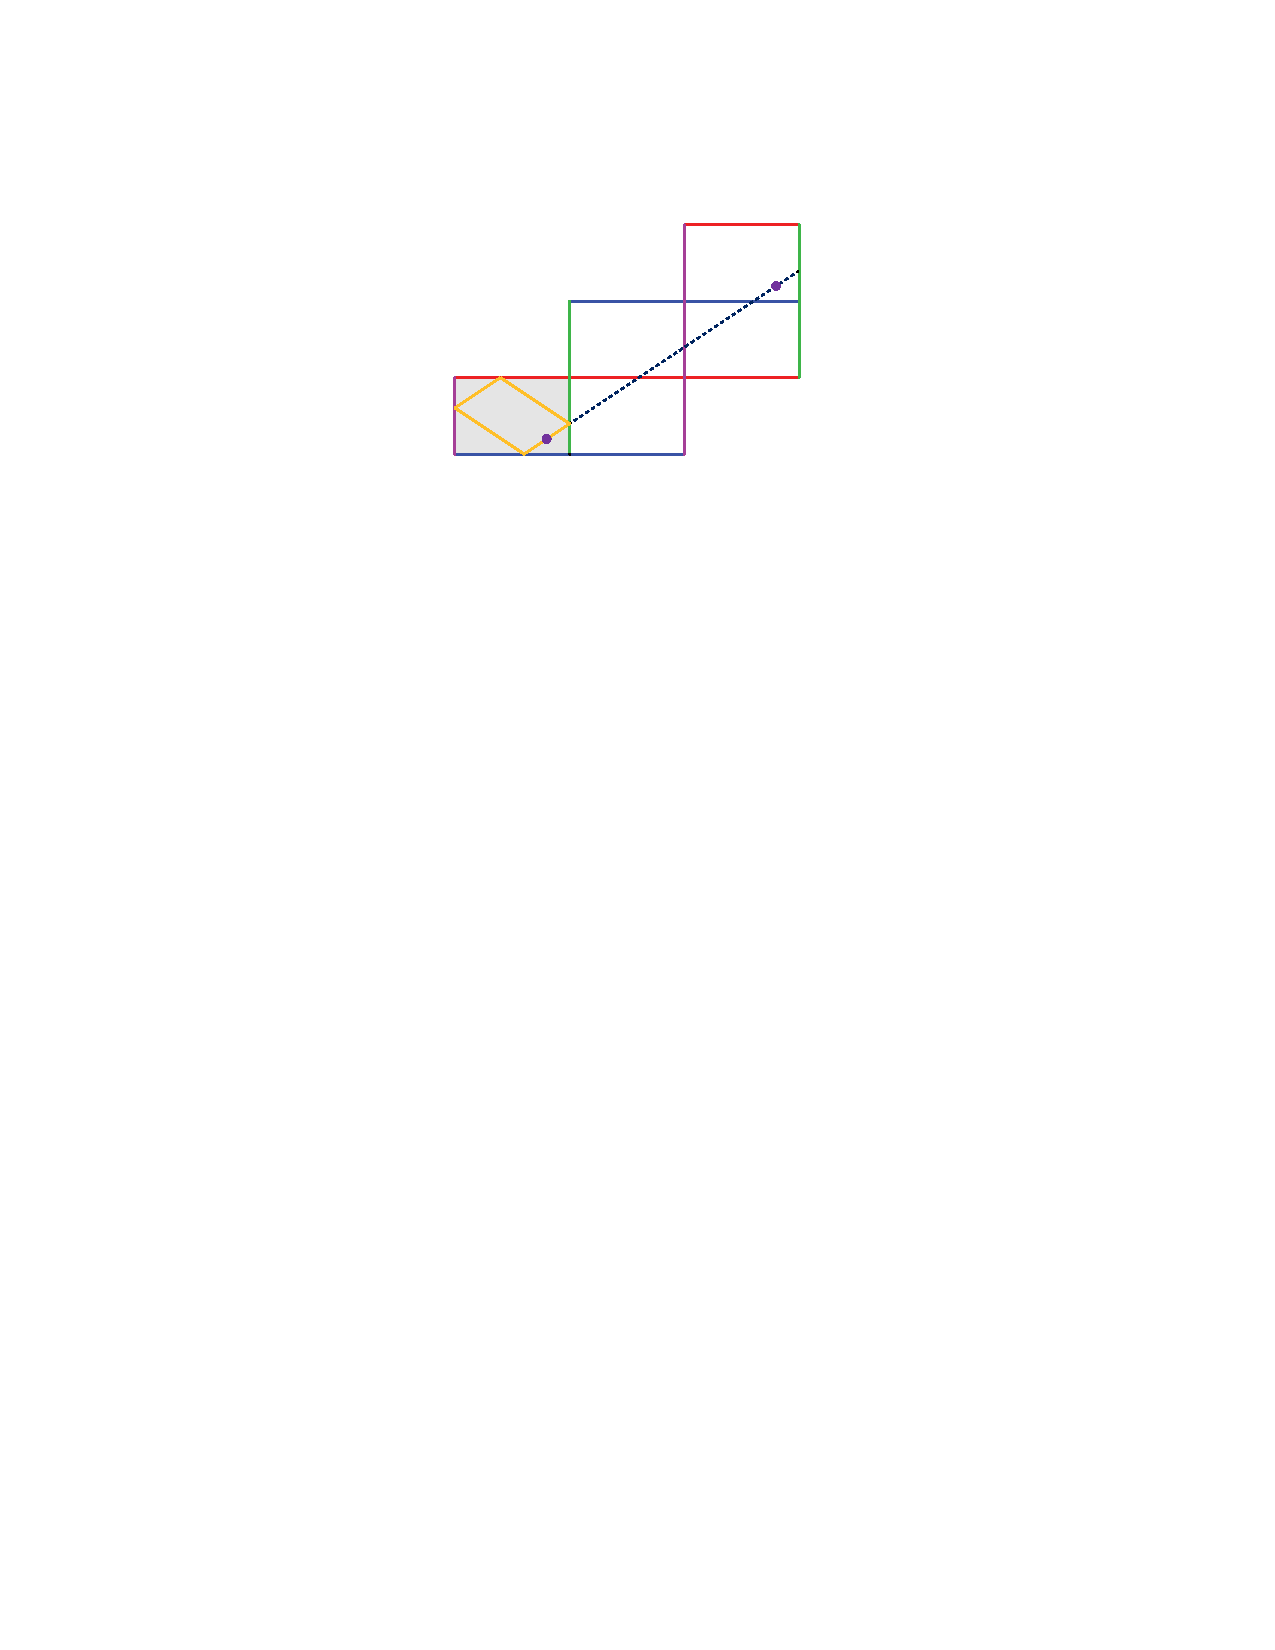
\includegraphics[width= 1\linewidth]{2}
		\caption{\small\textit{\color{duongvaotoanhoc}Hình $2$. Đường đi bi--a (liền nét)
		có thể được xem như một đường thẳng (đứt nét) trong mặt phẳng bằng cách liên tiếp lấy đối xứng bàn bi--a qua các cạnh của nó.}}
		\vspace*{-10pt}
	\end{figure}
	Hình chữ nhật là một đa giác đẹp bởi vì  bằng cách liên tiếp lấy đối xứng nó qua các cạnh, chúng ta có thể lát kín toàn bộ mặt phẳng. Nếu chúng ta làm điều này ngay từ đầu,
	thì mỗi đường thẳng trong mặt phẳng tương ứng với một đường đi bi--a trong hình chữ nhật (xem Hình $3$).
	\begin{figure}[H]
		\vspace*{-5pt}
		\centering
		\captionsetup{labelformat= empty, justification=centering}
		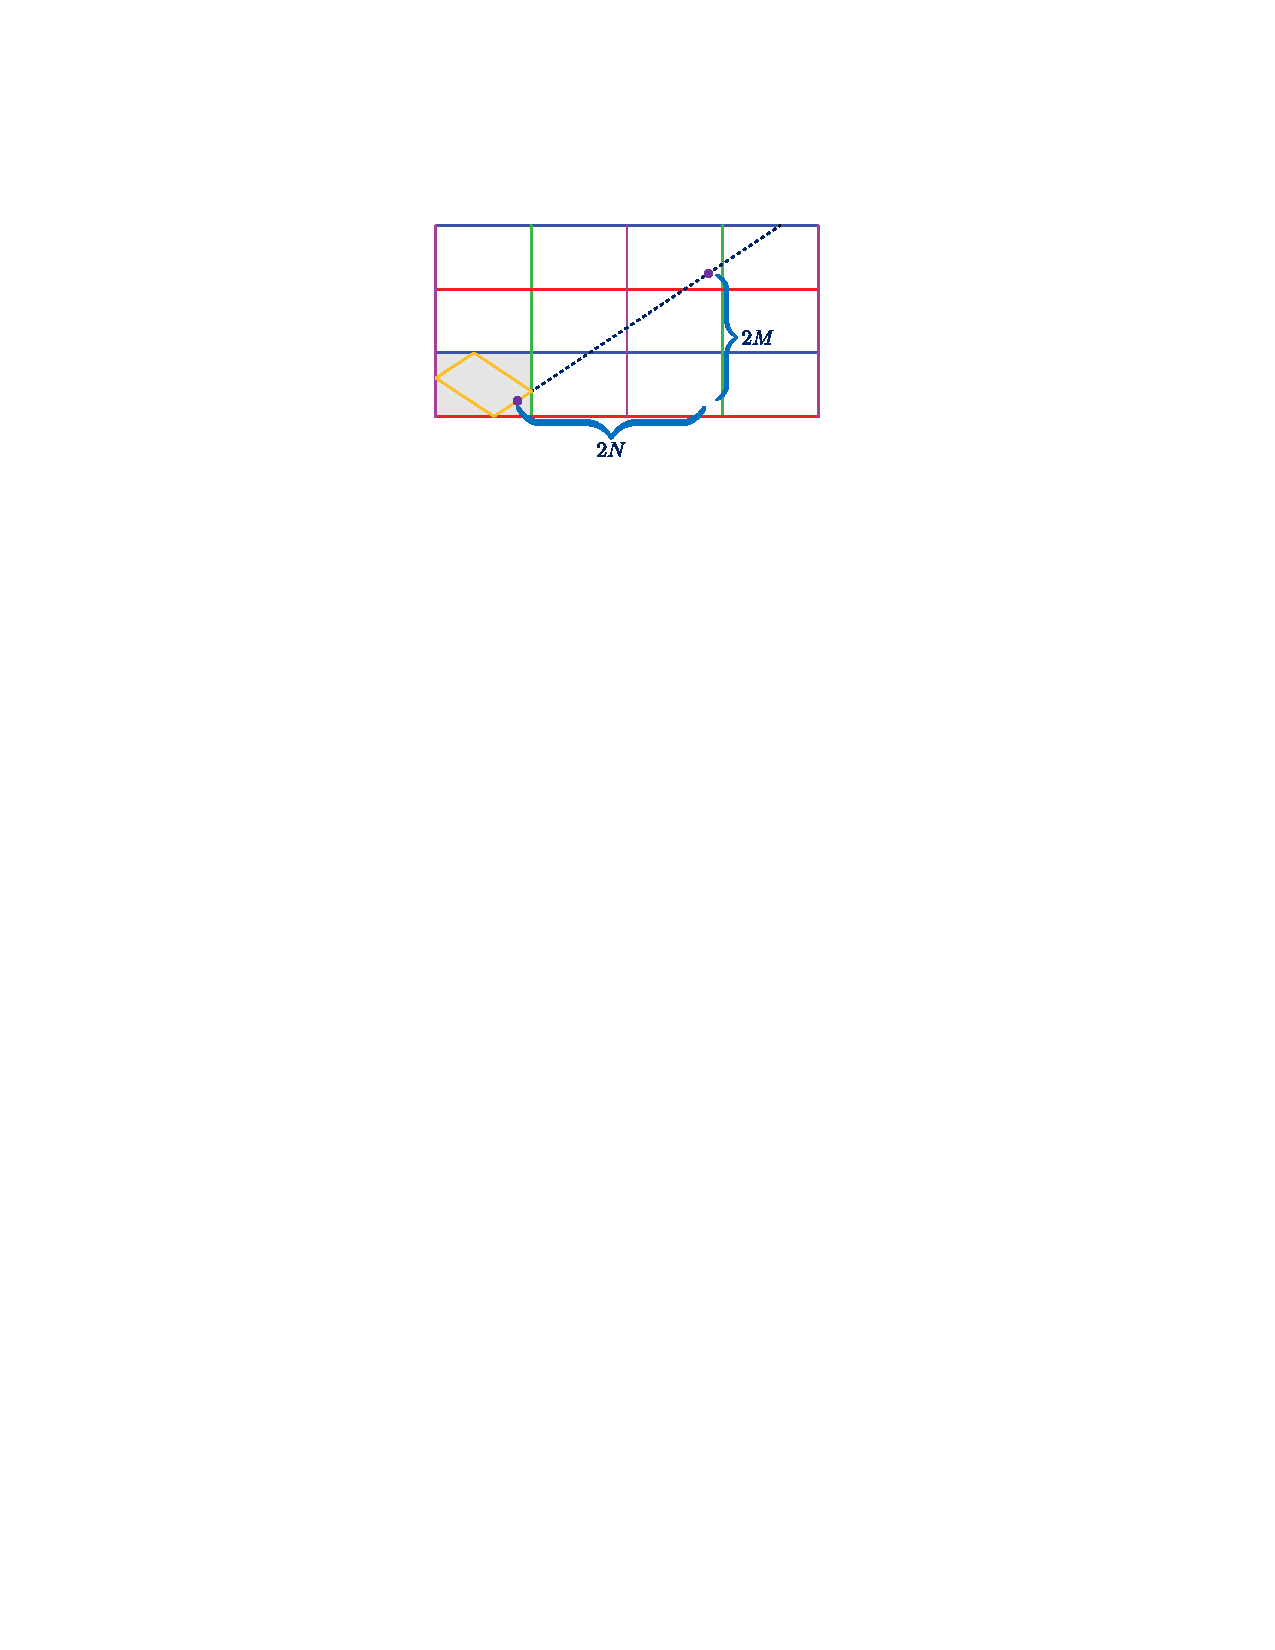
\includegraphics[width= 1\linewidth]{3}
		\caption{\small\textit{\color{duongvaotoanhoc}Hình $3$. Mặt phẳng được lát bằng bàn bi--a hình chữ nhật. Mỗi đường thẳng
		trong mặt phẳng tương ứng với một đường đi bi--a trên bàn.}}
		\vspace*{-10pt}
	\end{figure}
	Cho cặp số $(2N, 2M)$, chúng ta có thể tìm thấy một đường đi bi--a phản xạ theo cạnh ngang $2N$ lần và theo cạnh dọc $2M$ lần bằng cách vẽ một đường thẳng từ một điểm trong hình chữ nhật ban đầu đến điểm tương ứng trong hình chữ nhật mới nằm cách đó $2N$ bản sao theo chiều ngang và $2M$ bản sao theo chiều dọc. Như vậy ta đã tìm thấy mối quan hệ giữa các đường đi bi--a tuần hoàn và các cặp số nguyên không âm $(2N, 2M)$, chúng ta có định lý sau.
	\vskip 0.1cm
	{\bf\color{duongvaotoanhoc}Định lý.} Cho $R$ là một hình chữ nhật kích thước $a\times b$. Một đường đi bi--a trong $R$ là tuần hoàn khi và chỉ khi hệ số góc ban đầu của nó là một bội hữu tỷ của  $\frac{b}{a}.$
	\vskip 0.1cm
	Lưu ý rằng vị trí bắt đầu không đóng vai trò gì trong định lý này, vì vậy mỗi đường đi tuần hoàn thuộc một họ các đường đi tuần hoàn có cùng hệ số góc ban đầu.
	\vskip 0.1cm
	{\bf\color{duongvaotoanhoc}Bàn bi--a Tam giác}
	\vskip 0.1cm
	Trong trường hợp hình chữ nhật, chúng ta có hai tham số, $a$ và $b,$ để mô tả hình dạng của nó; sau khi suy xét, chúng ta nhận ra rằng chỉ \emph{lớp đồng dạng} của hình quyết định
	đường đi của bi--a. Điều này cho phép mô tả họ các hình chữ nhật bằng  một tham số duy nhất:
	tỉ số giữa $a$ và $b.$
	\vskip 0.1cm
	Trong trường hợp bàn tam giác, chúng ta có thể lấy ba số dương $a, b$ và $c$ bất kỳ thỏa mãn $a+b+c=180$ và tạo một tam giác với các góc bằng $a, b$ và $c$ (theo độ), với lớp đồng dạng được xác định duy nhất.
	Phương trình liên hệ giữa $a, b,$ và $c$ ngụ ý rằng chúng ta có một không gian hai tham số của các hình tam giác. 
	\vskip 0.1cm
	Trái ngược hoàn toàn với trường hợp hình chữ nhật, câu hỏi về những đường đi bi--a tuần hoàn nào  một tam giác cho trước có thể có (thậm chí ngay cả liệu nó có một đường nào hay không!) vẫn còn mở và là một lĩnh vực nghiên cứu sôi động. Chính xác hơn, chúng ta biết tất cả đường đi bi--a tuần hoàn cho một số loại tam giác. Đối với một số loại tam giác khác, chúng ta chỉ biết rằng tồn tại một  đường đi bi--a tuần hoàn. Nhưng đối với rất nhiều tam giác  khác, \emph{chúng ta không biết liệu có một đường đi bi--a tuần hoàn hay không!}
	\vskip 0.1cm
	Đừng thất vọng: với những hình tam giác quen thuộc nhất ở trường phổ thông--tam giác đều, tam giác $30-60-90$ và tam giác $45-45-90$, câu trả lời được biết rõ.
	\vskip 0.1cm
	Hãy thử chiến thuật mà chúng ta đã sử dụng với các hình chữ nhật, lấy đối xứng hình tam giác qua các cạnh của nó thay vì phản xạ  đường đi bi--a. Cũng thuận tiện giống như hình chữ nhật, ba hình tam giác này lát kín mặt phẳng như trong Hình $4$.  Các cạnh cùng màu tương ứng với cùng một cạnh của bàn bi--a. 
	\vskip 0.1cm
	Theo đúng cách mà chúng ta đã tìm thấy các đường đi bi--a tuần hoàn trong hình chữ nhật, chúng ta có thể nối các điểm tương ứng trong hai bản sao khác nhau của một tam giác trong phép lát để xây dựng các đường đi tuần hoàn. Bài tập: Đối với mỗi tam giác này, hãy xây dựng một định lý phân loại các đường đi bi--a tuần hoàn tương tự như định lý ở mục trước.
	\end{multicols}
	\begin{figure}[H]
		\vspace*{-5pt}
		\centering
		\captionsetup{labelformat= empty, justification=centering}
		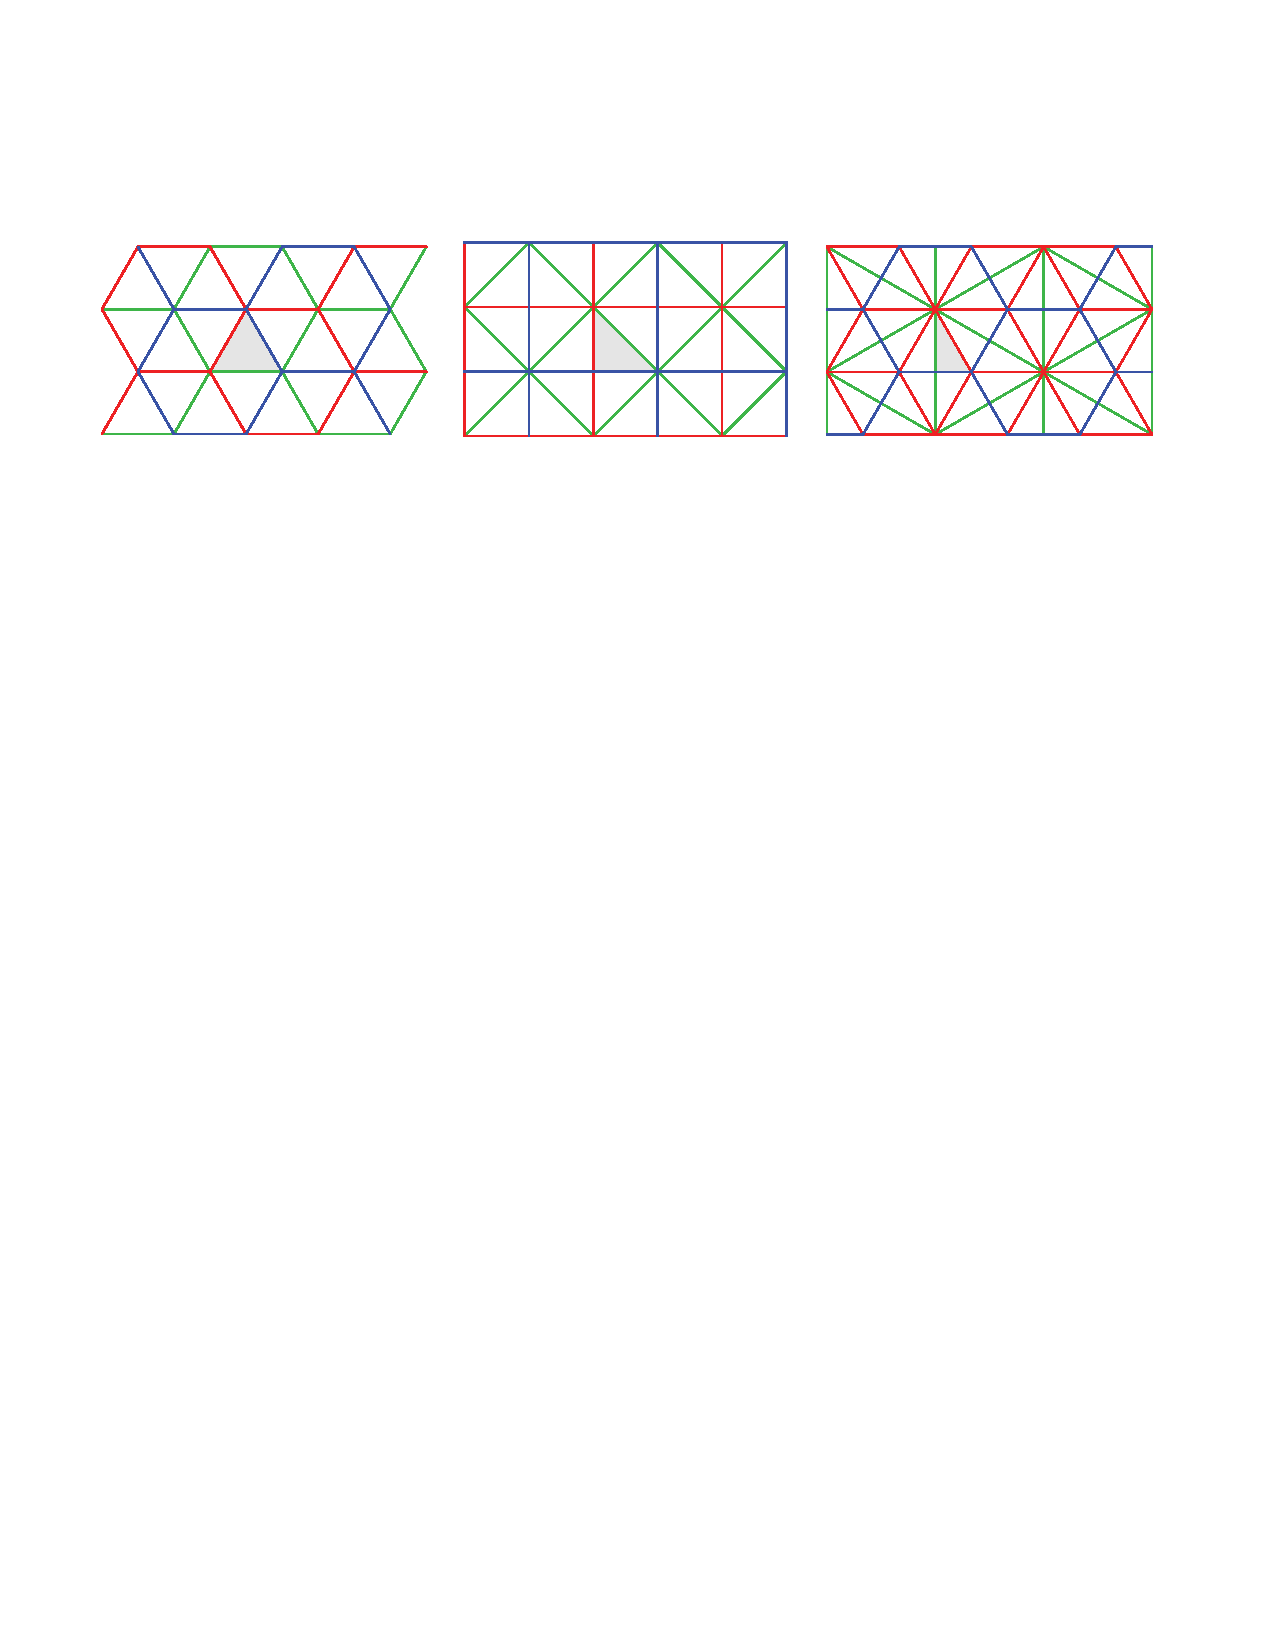
\includegraphics[width= 1\linewidth]{4}
		\caption{\small\textit{\color{duongvaotoanhoc}Hình $4$. Lát mặt phẳng bằng cách lấy đối xứng các tam giác đều, tam giác $45-45-90$ và tam giác $30-60-90$ qua các cạnh.}}
		\vspace*{-10pt}
	\end{figure}
	\begin{multicols}{2}
	Bây giờ, hãy giăng lưới của chúng ta rộng hơn ba loại tam giác đặc biệt này. Một trong những lớp đường đi bi--a tuần hoàn lâu đời nhất trong hình tam giác được Giovanni Fagnano tìm ra vào năm $1775$. Ông đã chứng minh rằng mọi tam giác \emph{nhọn} $T$ đều có một đường đi bi--a tuần hoàn. (Thật ra, khi đó ông  đang tìm kiếm  đường đi khép kín ngắn nhất chạm vào tất cả các cạnh, không nhất thiết phải tuân theo quy tắc phản xạ của bi--a, nhưng trong trường hợp này  đường đi ngắn nhất cũng chính là một  đường đi bi--a).
	\vskip 0.1cm
	Có thể xây dựng đường đi Fagnano một cách sơ cấp: Nối chân của ba đường cao trong tam giác (xem Hình $5$). Bài tập: chứng minh rằng
	tam giác này--được gọi là \emph{tam giác trực tâm} của $T$-- tạo thành một đường đi bi--a; tức là, chứng minh rằng mỗi cặp cạnh của
	tam giác trực tâm tạo với cạnh của $T$ các góc bằng nhau. Tại sao $T$ phải nhọn?
	\begin{figure}[H]
		\vspace*{-10pt}
		\centering
		\captionsetup{labelformat= empty, justification=centering}
		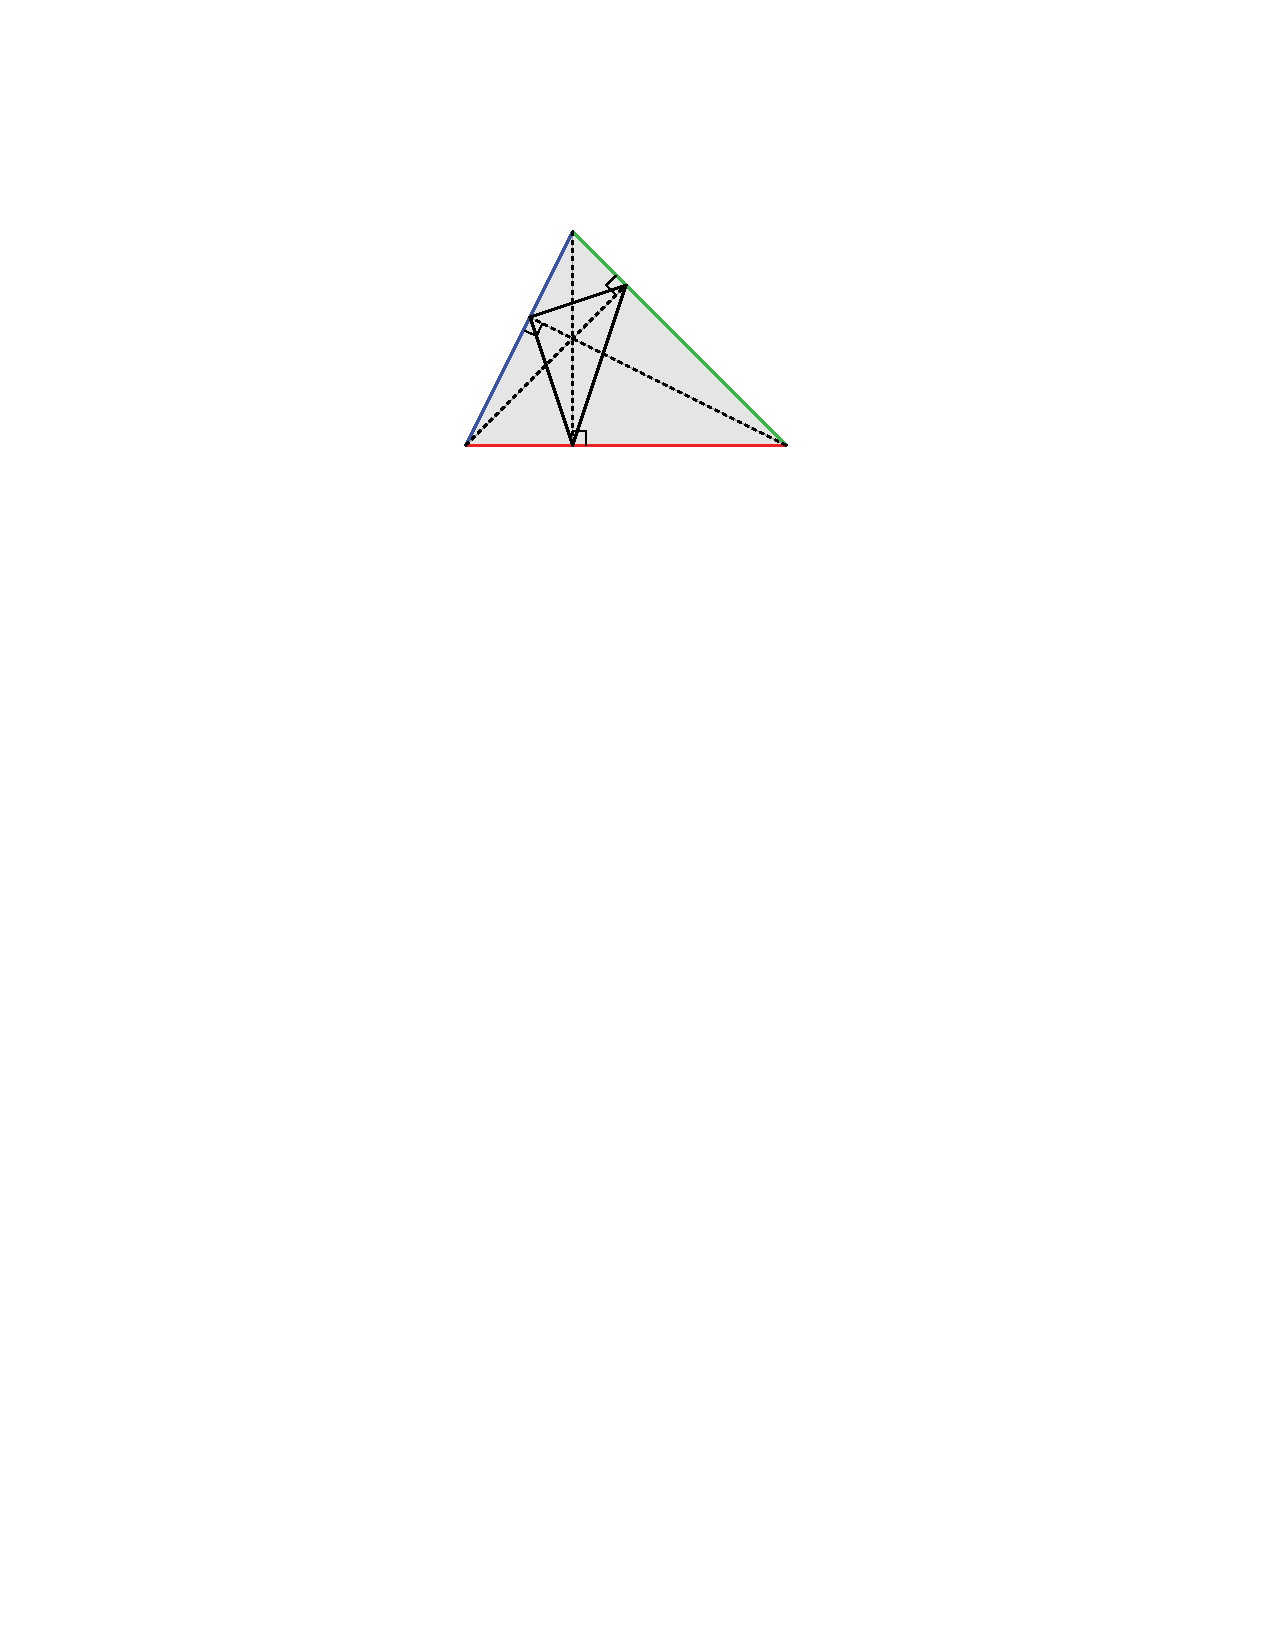
\includegraphics[width= 0.95\linewidth]{5}
		\caption{\small\textit{\color{duongvaotoanhoc}Hình $5$. Trong mọi tam giác nhọn, tam giác trực tâm tạo thành một đường đi bi--a tuần hoàn.}}
		\vspace*{-10pt}
	\end{figure}
	Từ đường đi tuần hoàn này, chúng ta nhận được thêm các đường đi tuần hoàn khác. Chỉ cần trải đường Fagnano ra. Bởi vì nó tuần hoàn, cuối cùng nó sẽ đến điểm tương ứng với vị trí xuất phát trong một bản sao có cùng hướng với tam giác $T$ ban đầu. Bất kỳ đường đi nào song song với đường đi ban đầu và nằm trong cùng một chuỗi  
	bản sao các tam giác chứa đường đi ban đầu cũng tuần hoàn. Xem Hình $6$ để thấy việc xây dựng này.
	\vskip 0.1cm
	Trong $30$ năm qua, đã có nhiều tiến bộ trong việc tìm kiếm các đường đi bi--a tuần hoàn trong tam giác. Đây là hai định lý minh họa cho những gì đã biết.
	\begin{figure}[H]
		\vspace*{-5pt}
		\centering
		\captionsetup{labelformat= empty, justification=centering}
		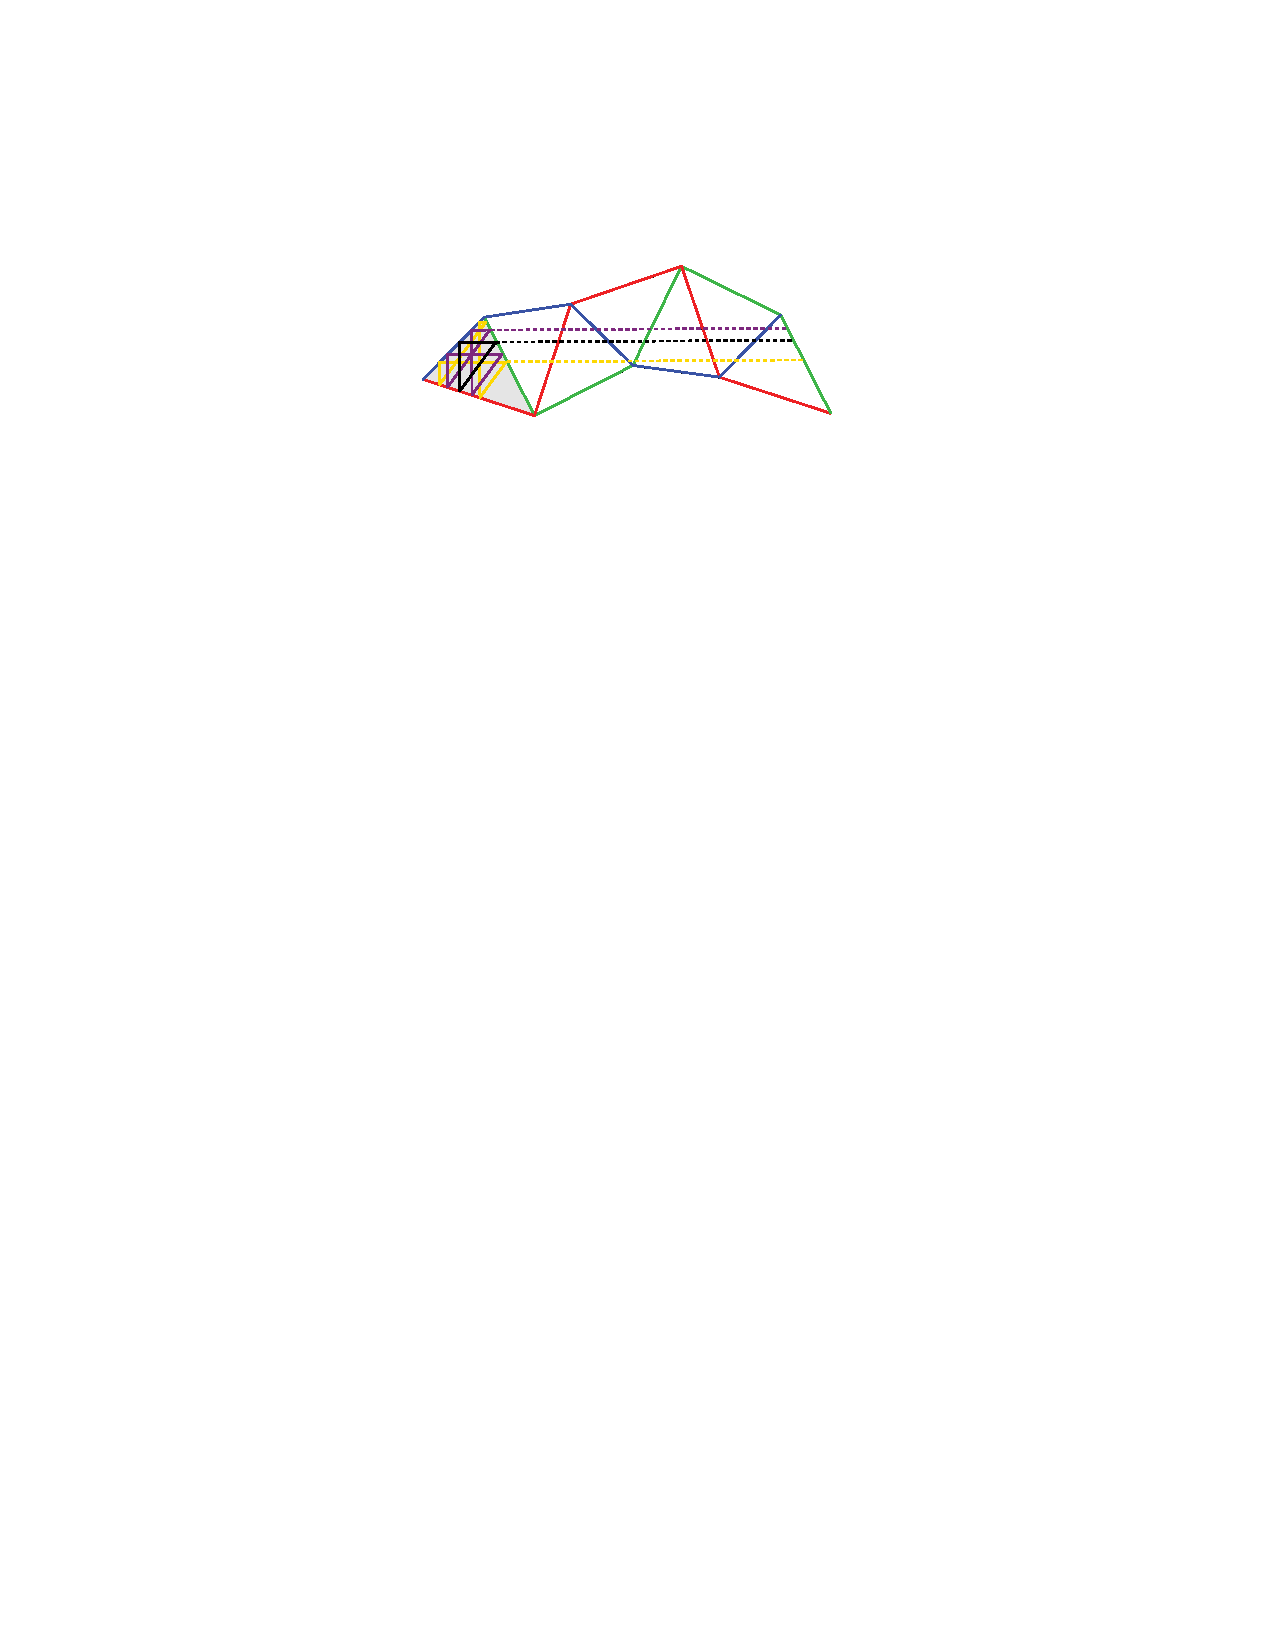
\includegraphics[width= 1\linewidth]{6}
		\caption{\small\textit{\color{duongvaotoanhoc}Hình $6$. Đường Fagnano màu đen, các đường màu tím, màu vàng song song với nó là các đường tuần hoàn mới.}}
		\vspace*{-10pt}
	\end{figure}
	{\bf\color{duongvaotoanhoc} Định lý} $\pmb{2.}$ Nếu số đo (theo độ) của tất cả các góc trong một tam giác đều là  số hữu tỷ thì tam giác đó có đường đi bi--a tuần hoàn theo vô số hướng.
	\vskip 0.1cm
	{\bf\color{duongvaotoanhoc} Định lý} $\pmb{3.}$ Mọi tam giác có các góc đều nhỏ hơn $100^{\circ}$ có một đường đi bi--a tuần hoàn.
	\vskip 0.1cm
	Cách chứng minh của hai định lý này hoàn toàn khác nhau. Định lý đầu tiên sử dụng các công cụ tiên tiến của giải tích phức  và tô-pô. Định lý thứ hai sử dụng tổ hợp, giải tích thực sơ cấp và cần sự hỗ trợ của máy tính.
	\vskip 0.1cm
	{\bf\color{duongvaotoanhoc}Điều gì tiếp theo?}
	\vskip 0.1cm
	Để đơn giản hóa vấn đề, chúng ta chỉ xét câu hỏi đường đi bi--a nào là tuần hoàn. Việc phân loại tính chất của các đường đi không tuần hoàn đòi hỏi phải đưa ra một loạt các khái niệm từ tô--pô và lý thuyết ergodic.
	\vskip 0.1cm
	Hơn nữa, chúng ta cũng mới chỉ xem xét hai hình dạng của bàn bi--a. Trường hợp bàn \linebreak bi--a hình đa giác tổng quát, đặc biệt là khi các
	góc có số đo hữu tỷ, cũng đang được nghiên cứu mạnh mẽ như trường hợp tam giác. Đây vẫn là một lĩnh vực nghiên cứu sôi động,
	với kho tàng kỹ thuật được sử dụng ngày càng gia tăng, được đúc kết từ nhiều chủ đề toán học khác nhau.
	\vskip 0.1cm
	Một số người đoạt huy chương Fields đã có những đóng góp mới và quan trọng trong việc nghiên cứu bi--a đa giác, bao gồm hai trong số những người nhận giải năm $2014$, Artur Avila (Người Brazil đầu tiên đoạt giải) và Maryam Mirzakhani (người phụ nữ đầu tiên và người Iran đầu tiên đoạt giải).
	\vskip 0.1cm
	Bi--a trong bàn có biên là đường cong (được gọi là bi--a trơn) tạo ra một màu sắc khác biệt; hình tròn và hình elip có các tính chất đẹp tương tự của hình chữ nhật. Để biết chi tiết về những điều này và những hệ bi--a trơn phức tạp hơn, độc giả có thể xem trong [$1$] và~[$4$].
	\vskip 0.1cm
	Mặc dù bi--a bắt đầu với những giả thiết đơn giản, nhưng nó đã phát triển thành một lý thuyết phong phú rút ra từ các lĩnh vực toán học dường như khác nhau. Đây thường là dấu hiệu của nghiên cứu toán học mới: Nó khám phá ra những mối liên hệ đáng kinh ngạc giữa các lĩnh vực khác nhau và sử dụng những mối liên hệ này để nhận được các kết quả mạnh mẽ về các đối tượng và quá trình đơn giản.
	\vskip 0.1cm
	{\bf\color{duongvaotoanhoc} Bi--a: Những khám phá toán học}
	\vskip 0.1cm
	Hai trong số bốn người nhận Huy chương Fields năm $2014$ đã có đóng góp đáng kể vào việc nghiên cứu bi--a đa giác. Ở đây chúng ta đưa ra những bản phác thảo ngắn gọn về công việc của họ trong lĩnh vực này. Trong cả hai trường hợp, nó sẽ giúp ta hiểu được mối liên hệ giữa bi--a đa giác và một đối tượng toán học được gọi là một \emph{mặt cong phẳng}.
	\vskip 0.1cm
	Từ đây trở đi, chúng ta đưa thêm một giả thiết rằng trong bàn bi--a đa giác của chúng ta tất cả các góc đều có số đo theo độ hữu tỷ. Chúng ta xây dựng mặt cong phẳng
	từ đa giác bằng cách sử dụng quá trình trải ra được mô tả trong mục trước: ta dán từng bản sao nhận được bằng cách lấy đối xứng đa giác vào bản sao trước đó. Khi tất cả
	các góc có số đo hữu tỷ, quá trình trải ra chỉ tạo ra được các bản sao quay đi theo một số hữu hạn các hướng khác nhau. Khi một bản sao của đa giác có cùng hướng với bản sao đã tạo ra,  chúng ta dán chúng với nhau. Ta làm như vậy với tất cả các cạnh của tất cả các bản sao đa~giác.
	\vskip 0.1cm
	Bằng cách này, chúng ta nhận được một mặt trừu tượng trông giống như mặt phẳng Euclid ở hầu hết các điểm (trừ những đỉnh của các đa giác). Đường đi bi--a trong
	đa giác trở thành các đường ``thẳng" trên mặt cong phẳng, và ngược lại. Hơn nữa, một đường đi bi--a tuần hoàn trong đa giác tương ứng với một vòng khép kín, đi thẳng trên
	mặt cong phẳng.
	\begin{figure}[H]
		\vspace*{-10pt}
		\centering
		\captionsetup{labelformat= empty, justification=centering}
		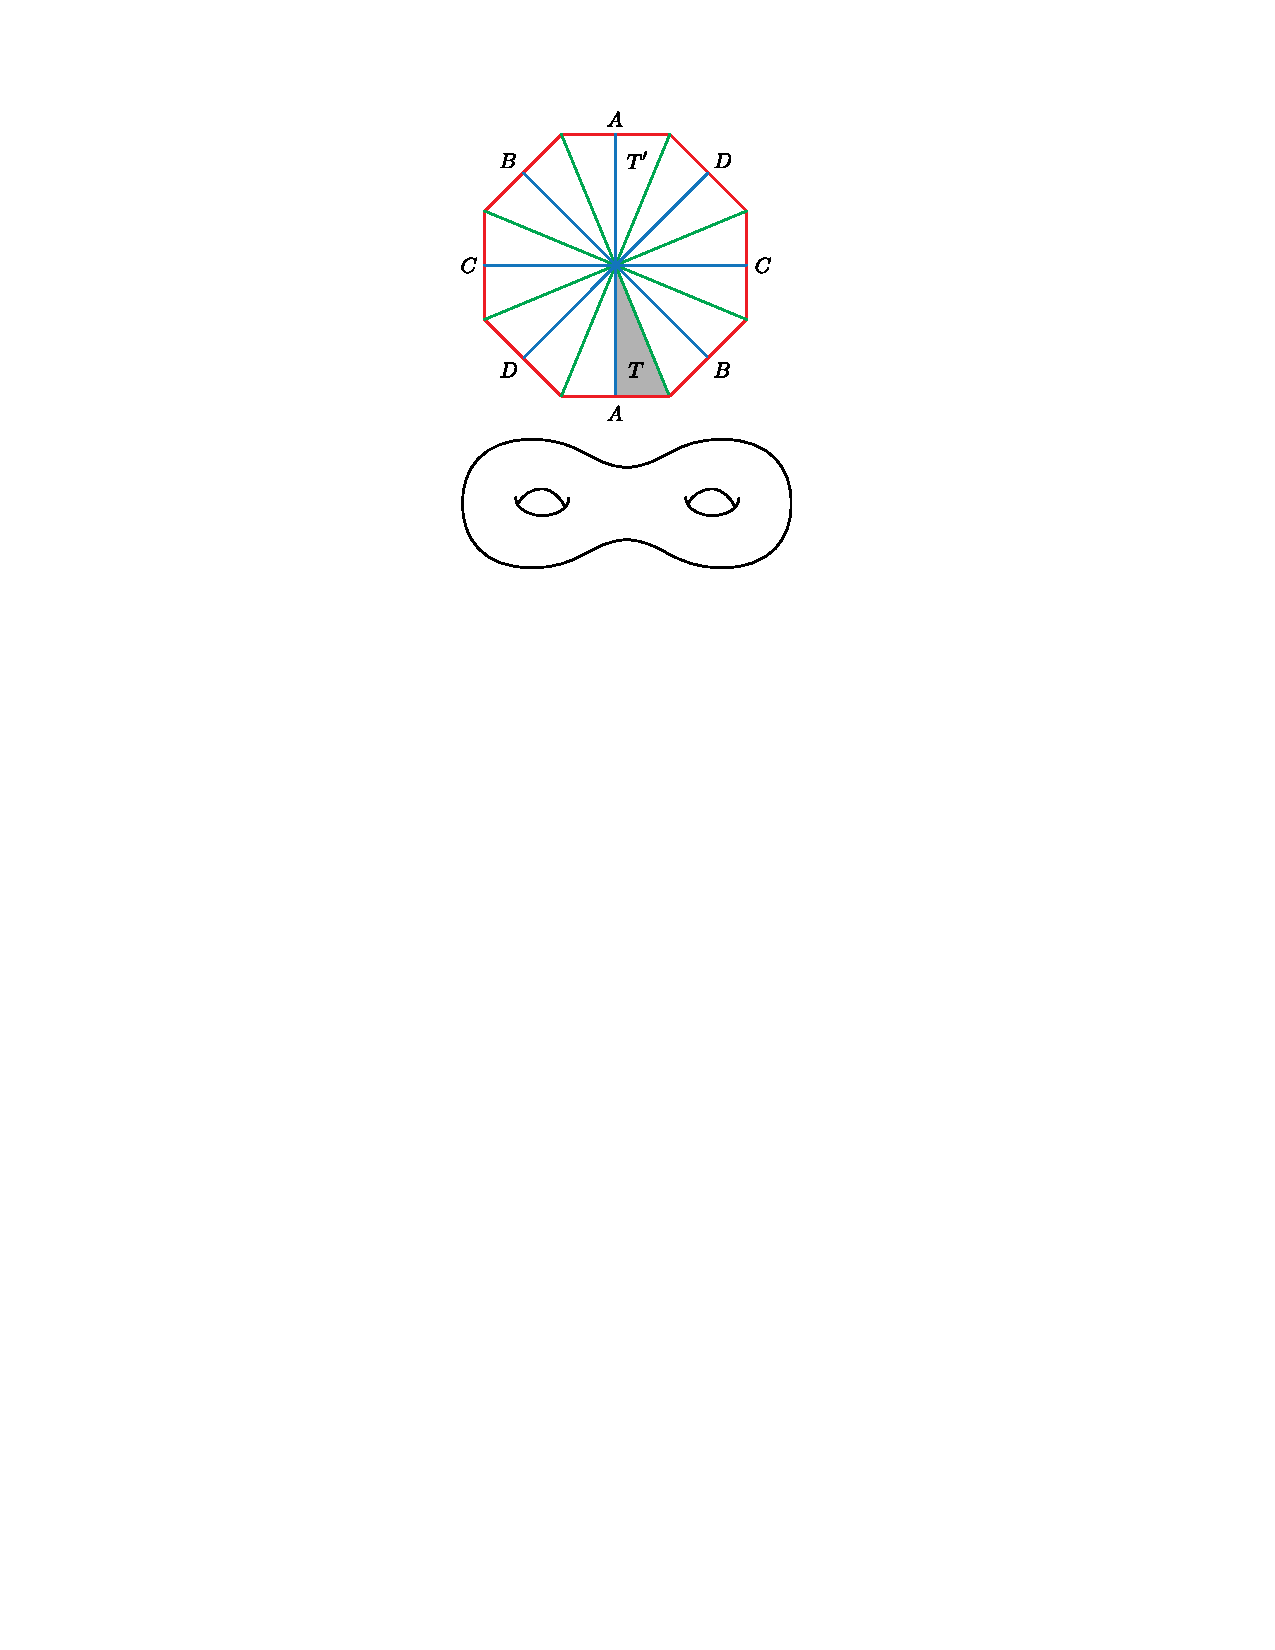
\includegraphics[width= 1\linewidth]{7}
		\caption{\small\textit{\color{duongvaotoanhoc}Hình $7$. Trải tam giác $T$ ra thành một hình bát giác đều. Mỗi cặp cạnh có cùng tên được dán lại với nhau để tạo  một mặt cong phẳng có cấu trúc tô-pô như một hình xuyến có hai quai.}}
		\vspace*{-10pt}
	\end{figure}
	Chúng ta hãy xét ví dụ một tam giác vuông $T$ với một bằng góc $22,5^{\circ}$ (xem hình $7$). Trải nó ra để nhận được một hình bát giác đều. Khi lấy đối xứng bất kỳ bản sao nào trong số $16$ bản sao này, chúng ta sẽ lại nhận được một trong số chúng. Ví dụ, nếu lấy đối xứng tam giác $T$ qua cạnh màu đỏ của nó, chúng ta nhận được tam giác $T'.$ Vì vậy, chúng ta nhận được một mặt cong phẳng bằng cách dán các cạnh $A$ với $A$, $B$ với $B$, $C$ với $C$, và $D$ với $D.$
	\vskip 0.1cm
	Về mặt trực quan, điều này có nghĩa là một đường đi ``rời khỏi" bát giác ở một cạnh bên sẽ đi vào điểm tương ứng trên cạnh cùng tên của chính mặt đó. Bài tập: thuyết phục bản thân rằng mặt cong phẳng này tương đương tô-pô với hình xuyến hai quai. Đây là một phiên bản phức tạp hơn của hình xuyến một quai quen thuộc thu được từ việc dán các cạnh đối diện của một hình vuông.
	\vskip 0.1cm
	Các mặt cong phẳng khác có thể thu được từ các đa giác bằng cách dán các cạnh song song mà ta chọn lại với nhau, không nhất thiết phải theo một quá trình lấy đối xứng. Ví dụ, chúng ta có thể đơn giản là bắt đầu ngay với hình bát giác trong Hình $7$, chứ không cần trải tam giác ra. Tập hợp tất cả các mặt cong phẳng có một khái niệm tự nhiên về sự gần--xa: Hai mặt cong là \emph{gần nhau} nếu chúng được xây dựng từ các hình đa giác mà chỉ cần một biến dạng nhỏ là có thể biến đổi từ hình này thành hình kia.
	\vskip 0.1cm
	{\bf\color{duongvaotoanhoc}Artur Avila}
	\vskip 0.1cm
	Công việc mà Artur Avila theo đuổi thường tìm cách mô tả dáng điệu \emph{điển hình} trong các hệ động lực--nghĩa là, trả lời câu hỏi về điều gì sẽ xảy ra ``trong hầu hết toàn bộ thời gian." Các đường đi tuần hoàn trong bàn bi--a là cực kỳ \emph{không điển hình}, giống như việc các số hữu tỷ là không điển hình trong tập số thực. Hầu hết các đường đi bi--a theo thời gian sẽ đến gần mọi điểm trên bàn, một khoảng cách nhỏ tùy ý (theo thuật ngữ tô-pô, hầu hết các đường đi là \emph{trù mật} trên bàn).
	Đây chỉ là một phần của kết quả; chúng ta cũng có thể đặt câu hỏi đường đi bao phủ bàn bi--a nhanh như thế nào. Câu trả lời cho những câu hỏi như vậy có thể phát biểu dễ dàng hơn trên mặt con phẳng tương ứng.
	\vskip 0.1cm
	Avila chứng minh, trong công trình chung với Giovanni Forni, với hầu hết các mặt cong phẳng, chuyển động theo đường thẳng là \emph{trộn yếu}. Có thể hình dung tính chất này như sau: Giả sử một vùng $P$ bao phủ $p\%$ của mặt cong và tất cả các điểm trong $P$ bắt đầu di chuyển theo cùng một hướng. Khi đó, với hầu hết mọi hướng ban đầu và bất kỳ vùng $R$ nào, đến một lúc nào đó, tính trung bình,  các điểm xuất phát từ $P$ sẽ bao phủ $p\%$ của $R.$ Do đó, một quả bóng sẽ được phân tán đều khắp trên mặt cong, ngay cả khi  ban đầu nó chỉ tập trung ở
	một vùng. Tuy nhiên, các mặt cong  phẳng xuất phát từ bi--a là không điển hình, và vì vậy kết quả nói trên không cho hệ quả trực tiếp nào liên quan đến bi--a.
	\begin{figure}[H]
		\vspace*{-5pt}
		\centering
		\captionsetup{labelformat= empty, justification=centering}
		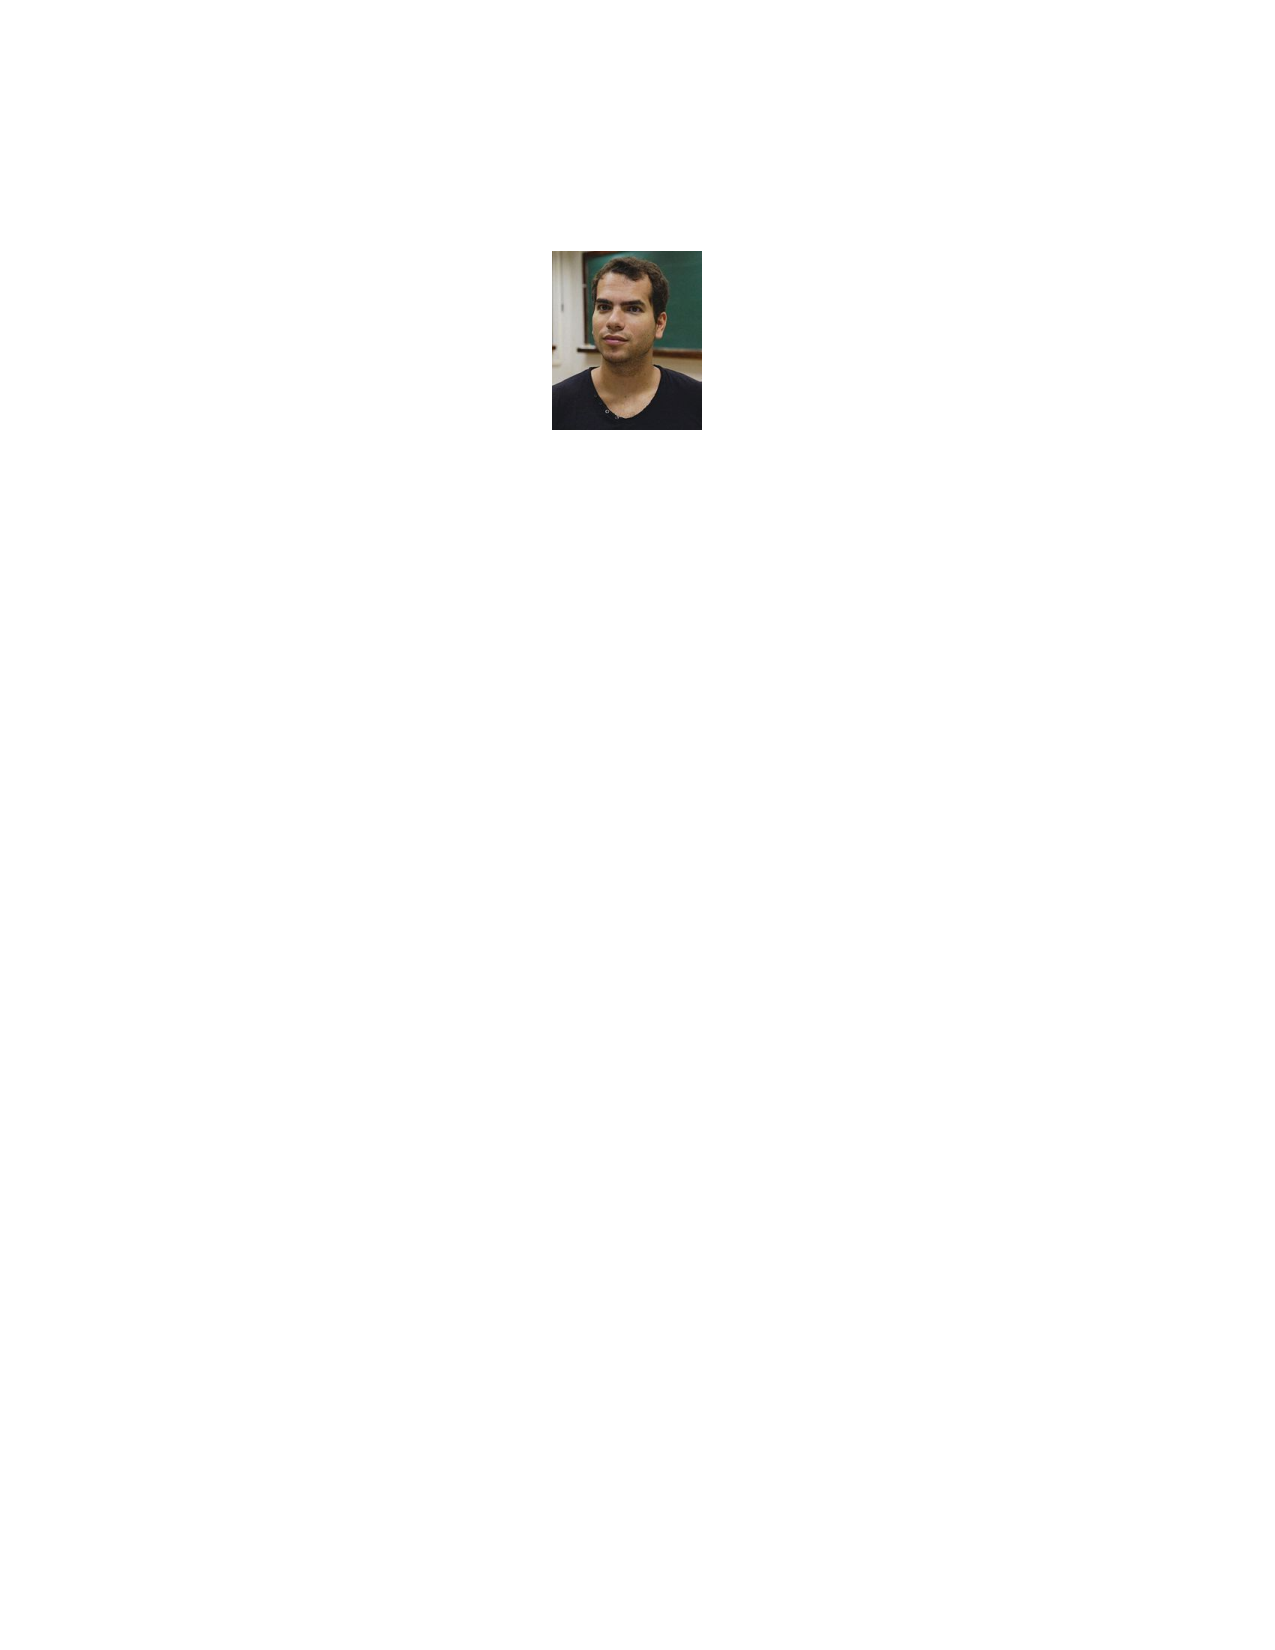
\includegraphics[width= 0.85\linewidth]{8}
		\vspace*{-10pt}
	\end{figure}
	Tuy nhiên, bàn bi--a cho phép xây dựng hiển các mặt cong có tính chất trộn yếu. Như Avila thể hiện trong công trình sau đó, với Vincent Delecroix, tính trộn yếu không chỉ đúng đối với các  mặt cong điển hình, mà còn đúng với các trường hợp cụ thể của các mặt cong nhận được từ đa giác đều (như trong Hình $7$), ngoại trừ hình tam giác, hình vuông,
	hoặc hình lục giác.
	\vskip 0.1cm
	Cuối cùng, Avila, cùng với Marcelo Viana, chứng tỏ rằng trên một mặt cong phẳng điển hình, độ lệch của một đường thẳng điển hình so với dáng điệu tiệm cận khi uốn lượn quanh bề mặt của nó  có thể được mô tả một cách chính xác (điều gọi là \emph{hiện tượng Zorich}). 
	\vskip 0.1cm
	Các chi tiết khác về công việc của Avila về các mặt cong phẳng có thể được tìm thấy trong bài báo của Forni ``Về công trình đoạt giải Brin của
	Artur Avila trong Động lực học Teichmüller và các phép trao đổi đoạn thẳng", được xuất bản trên Tạp chí Động lực học Hiện đại (Journal
	of Modern Dynamics) năm $2012$.
	\vskip 0.1cm
	{\bf\color{duongvaotoanhoc}Maryam Mirzakhani}
	\vskip 0.1cm
	Công việc của Maryam Mirzakhani liên quan trực tiếp hơn đến các cách mà mặt cong  phẳng có thể bị biến dạng. Nhắc lại, điều này có nghĩa là làm biến dạng các đa giác được sử dụng để tạo
	ra mặt đó. Một loại biến dạng cụ thể như vậy thay đổi tất cả đa giác đồng thời bằng một phép biến đổi tuyến tính--nghĩa là, bằng cách tác động một ma trận khả nghịch vào các đa giác để tạo ra các hình dạng mới.
	\begin{figure}[H]
		%		\vspace*{-5pt}
		\centering
		\captionsetup{labelformat= empty, justification=centering}
		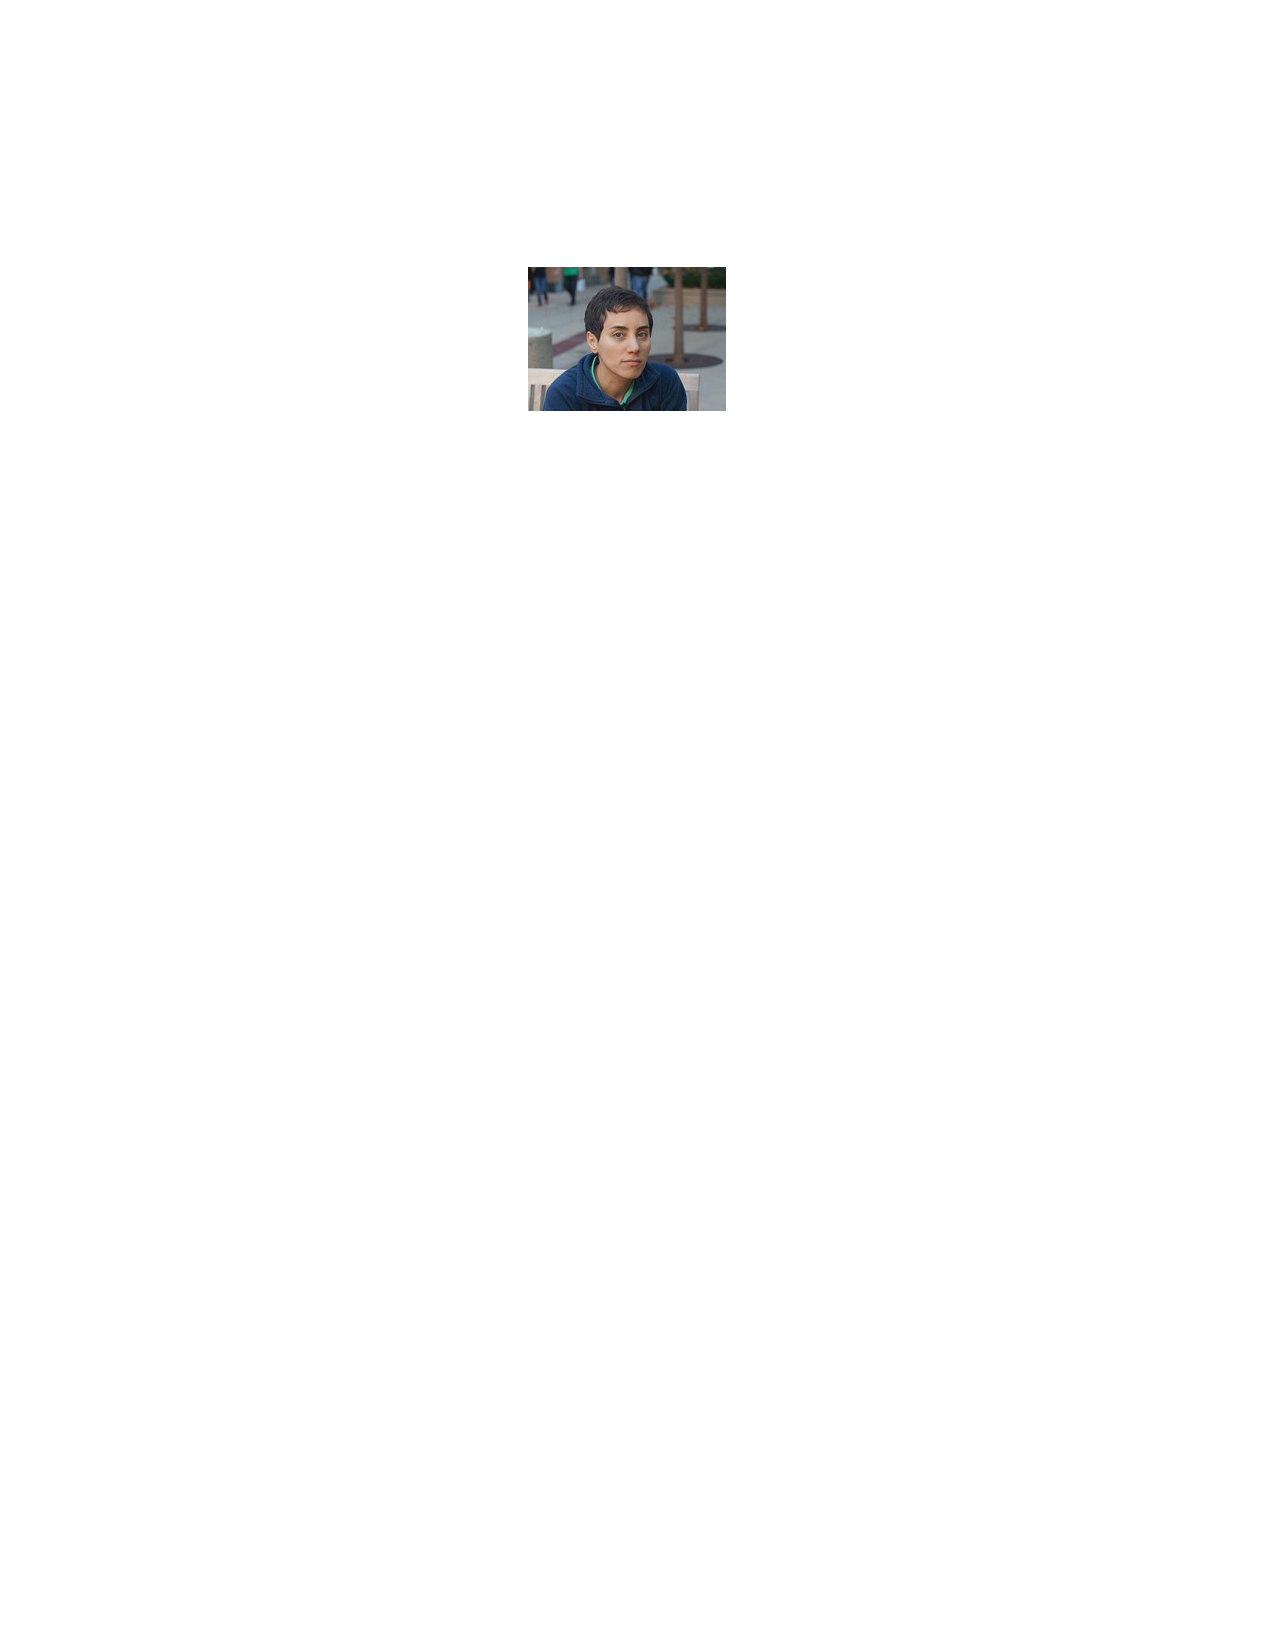
\includegraphics[width= 1\linewidth]{9}
		\vspace*{-15pt}
	\end{figure}
	Mirzakhani, trong công trình chung với Alex Eskin và Amir Mohammadi, đã nghiên cứu tập hợp các mặt cong có thể được xấp xỉ gần đúng bằng cách biến đổi tuyến tính một mặt ban đầu (quan điểm này là nền tảng cho nhiều kết quả đã nêu ở các mục trước và trong công trình của Avila). Trong không gian các mặt cong phẳng, tập hợp con này có thể là rất phức tạp--chẳng hạn như có dạng fractal.
	\vskip 0.1cm
	Tuy nhiên, Mirzakhani và các cộng sự của cô ấy đã cho thấy rằng nó luôn rất tốt: Nó có thể được mô tả (địa phương) bằng các phương trình \emph{tuyến tính} trong tọa độ của
	các đa giác tạo nên mặt cong phẳng. Trước đây, trường hợp không tầm thường duy nhất mà điều này đúng là của hình xuyến $2$ chiều, trong công trình của Curtis McMullen (đoạt giải Fields năm $1998$).
	\vskip 0.1cm
	Một điều ngạc nhiên là điều kiện về mặt cong nào có thể được xấp xỉ gần đúng bằng cách biến dạng tuyến tính của mặt ban đầu lại mang thông tin về động lực học của các đường thẳng trên mặt ban đầu. Do đó, công việc được mô tả trong đoạn văn trước cho hệ quả về các đường đi bi--a--bao gồm cả các đường đi bi--a tuần hoàn--chỉ mới bắt đầu được khám phá.
	\vskip 0.1cm
	Các chi tiết khác về công trình của Mirzakhani về các mặt cong phẳng có thể được tìm thấy trong bài báo cáo của McMullen tại Đại hội Toán học Thế giới ``Công trình Toán học của Maryam Mirzakhani", có trên trang web cá nhân của ông (\url{http://bit.ly/1DyH3Ha}).
	\vskip 0.1cm
	{\bf\color{duongvaotoanhoc}Tài liệu đọc thêm}
	\vskip 0.1cm
	[$1$] Leonid Bunimovich, ``Dynamical billiards," {\it Scholarpedia} $2$, no. $8$ ($2007$): $1813$.
	\vskip 0.1cm
	[$2$] Howard Masur, ``Closed trajectories for quadratic differentials with an application to billiards," {\it Duke Math. J.} $53$, no. $2$ ($1986$): $307-314$.
	\vskip 0.1cm
	[$3$] Richard Schwartz, ``Obtuse triangular billiards II:$100$ degrees worth of periodic trajectories," {\it Experimental Mathematics} $18$, no. $2$ ($2008$): $137-171$.
	\vskip 0.1cm
	[$4$] Serge Tabachnikov, {\it Geometry and Billiards}, Providence, RI: American Mathematical Society, $2005$.
\end{multicols}
